% !TeX document-id = {9187d367-de56-4c98-b3e5-bfd8c84fd026}
% !TeX TXS-program:compile = txs:///pdflatex/[--shell-escape]
\documentclass[12pt, a4paper]{article}
\usepackage[a4paper, total={6in, 8in}]{geometry}
\usepackage[english]{babel}
\usepackage[utf8]{inputenc}
\usepackage{multirow}
\usepackage{calc}
\usepackage{array}
\usepackage{caption} 
\captionsetup[table]{skip=5pt}
\usepackage{graphicx}
\usepackage{enumitem}
\usepackage{natbib}
\usepackage{minted}

\newlength\celldim
\setlength\celldim{2.5em}
\newlength\fontheight
\settoheight\fontheight{A}
\newlength\extraheight
\setlength\extraheight{\celldim - \fontheight}

\setlist[itemize]{leftmargin=*}

\makeatletter
\newcolumntype{S}
{ @{}
	>{\centering\arraybackslash}
	p{\celldim}
	<{\rule[-0.5\extraheight]{0pt}%
		{\fontheight + \extraheight}}
	@{} }
\makeatother


\title{Planning: \\Heuristic Analysis}
\author{Raphael Ballet}
\date{}

%Provide an optimal plan for Problems 1, 2, and 3.
%Compare and contrast non-heuristic search result metrics (optimality, time elapsed, number of node expansions) for Problems 1,2, and 3. Include breadth-first, depth-first, and at least one other uninformed non-heuristic search in your comparison; Depth-first may be skipped for Problem 3 if it takes longer than 10 minutes to run, but a note in this case should be included.
%Compare and contrast heuristic search result metrics using A* with the "ignore preconditions" and "level-sum" heuristics for Problems 1, 2, and 3.
%What was the best heuristic used in these problems? Was it better than non-heuristic search planning methods for all problems? Why or why not?
%Provide tables or other visual aids as needed for clarity in your discussion.

\begin{document}
	\maketitle
	
	This work presents the results of the ''Planning Search'' project. It uses several search methods with different heuristics to solve the air cargo problem defined in classical PDDL (Planning Domain Definition Language).
	
	\section{Air Cargo Problems}
	
	The aircargo action schema is shown bellow. It is used for all three air cargo problems.
	
\begin{center}
	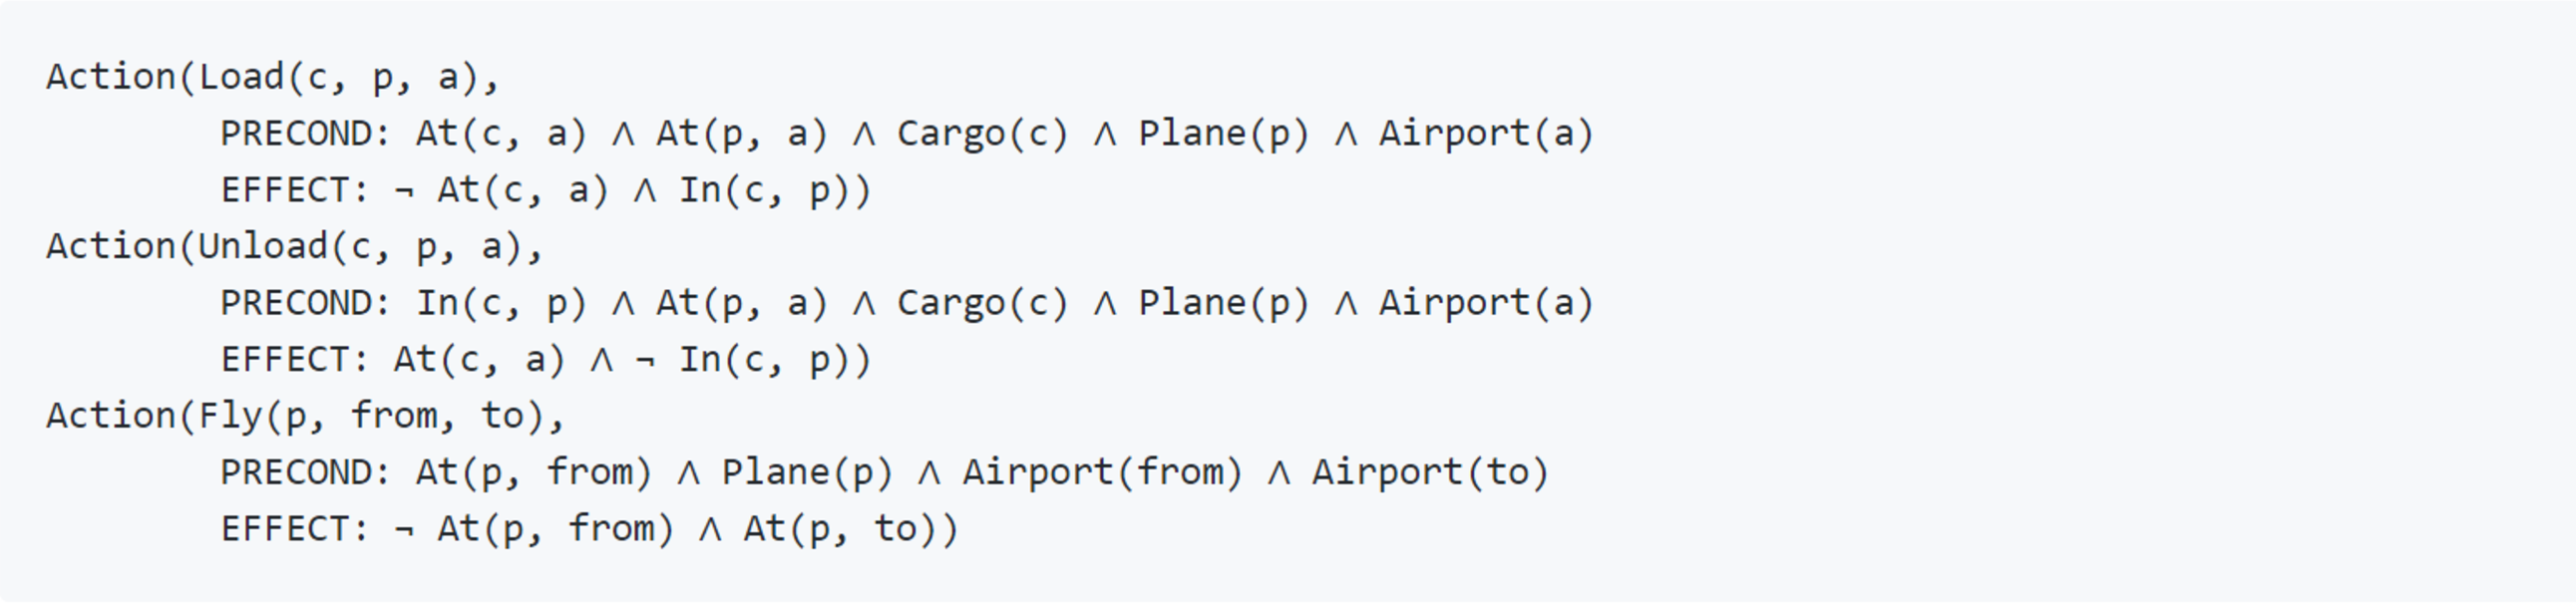
\includegraphics[width=1\linewidth]{action_schema}
\end{center}

	Each air cargo problem differs from one another only in the definition of its initial state and objective.
	
	\begin{itemize}
		\item Problem 1:
		\begin{center}
			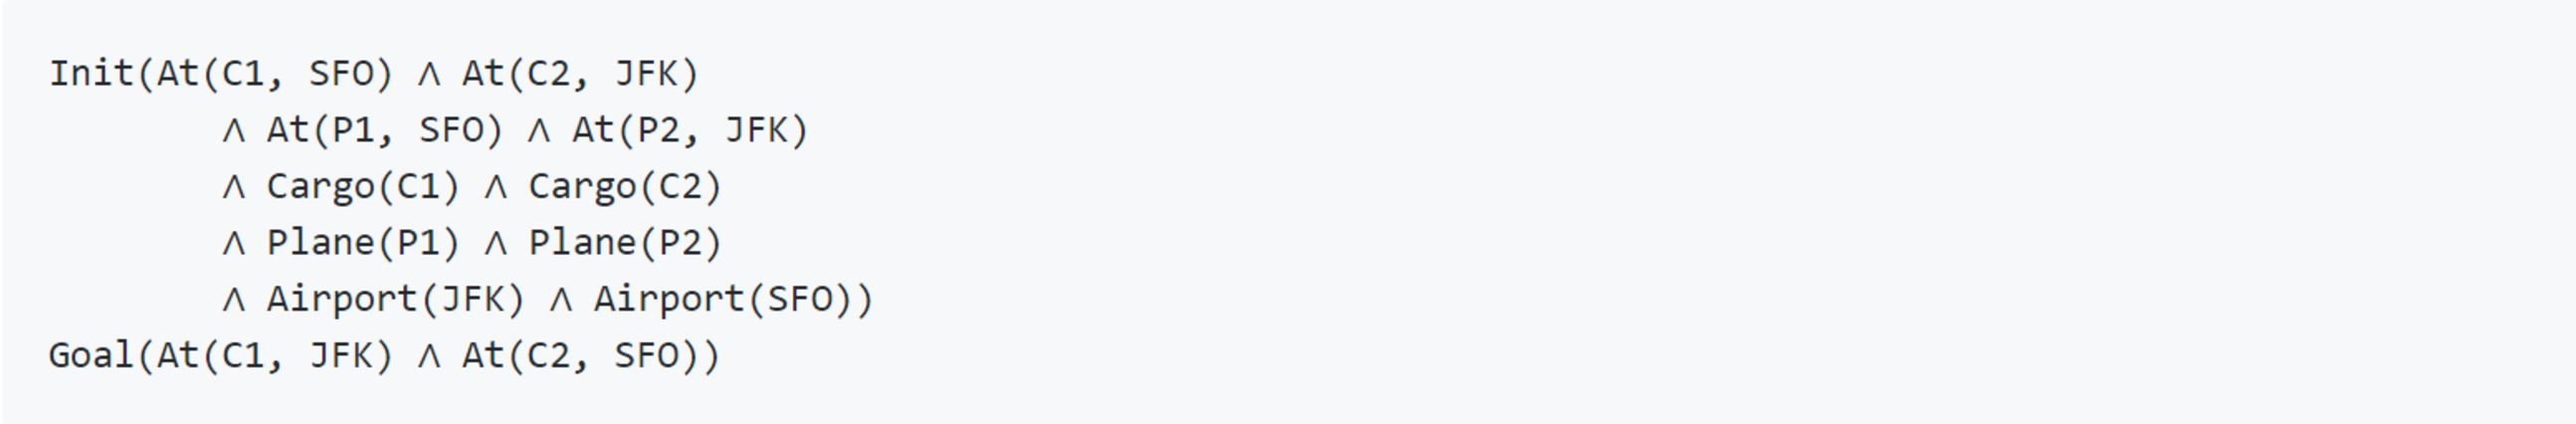
\includegraphics[width=1\linewidth]{problem_1}
		\end{center}
	\pagebreak
		\item Problem 2:
		\begin{center}
			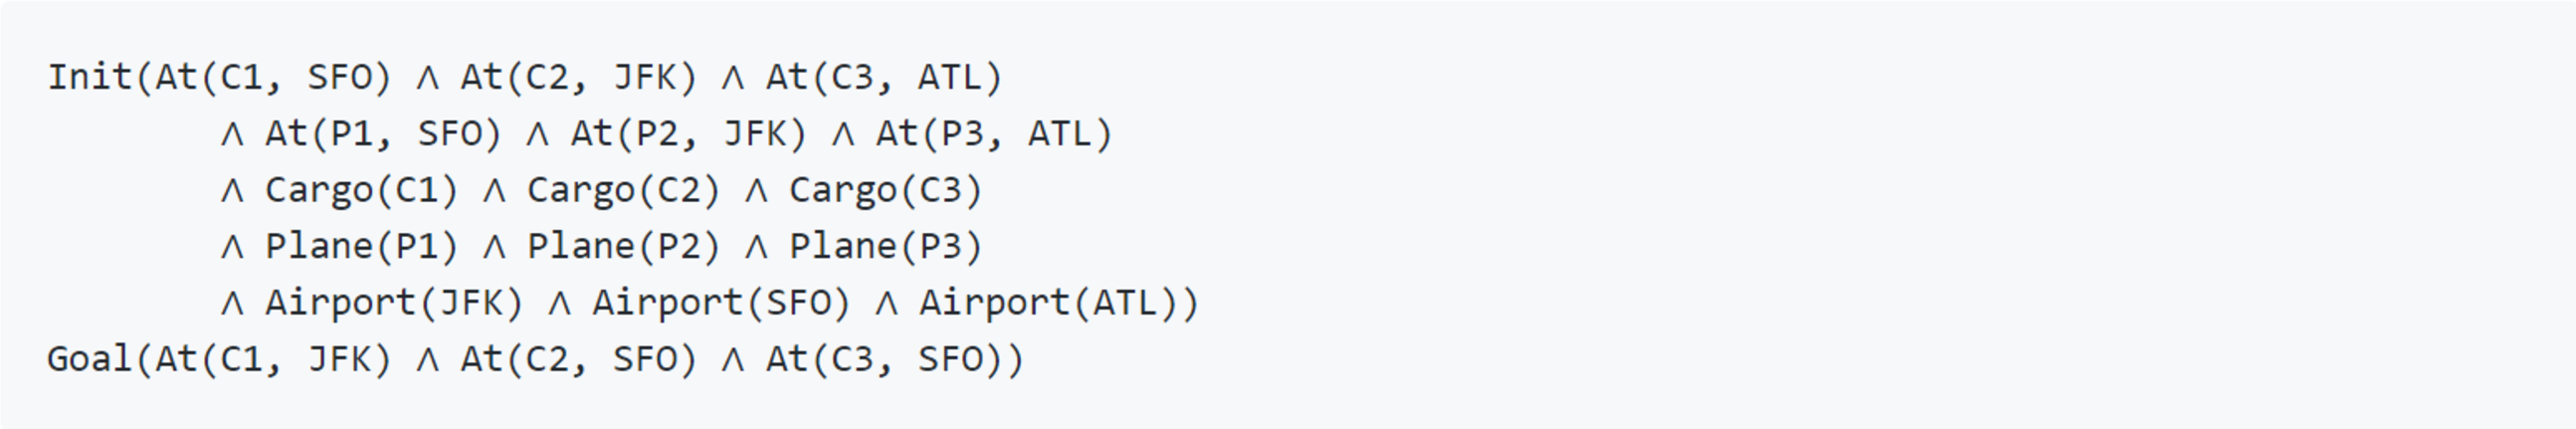
\includegraphics[width=1\linewidth]{problem_2}
		\end{center}
		\item Problem 3:
		\begin{center}
			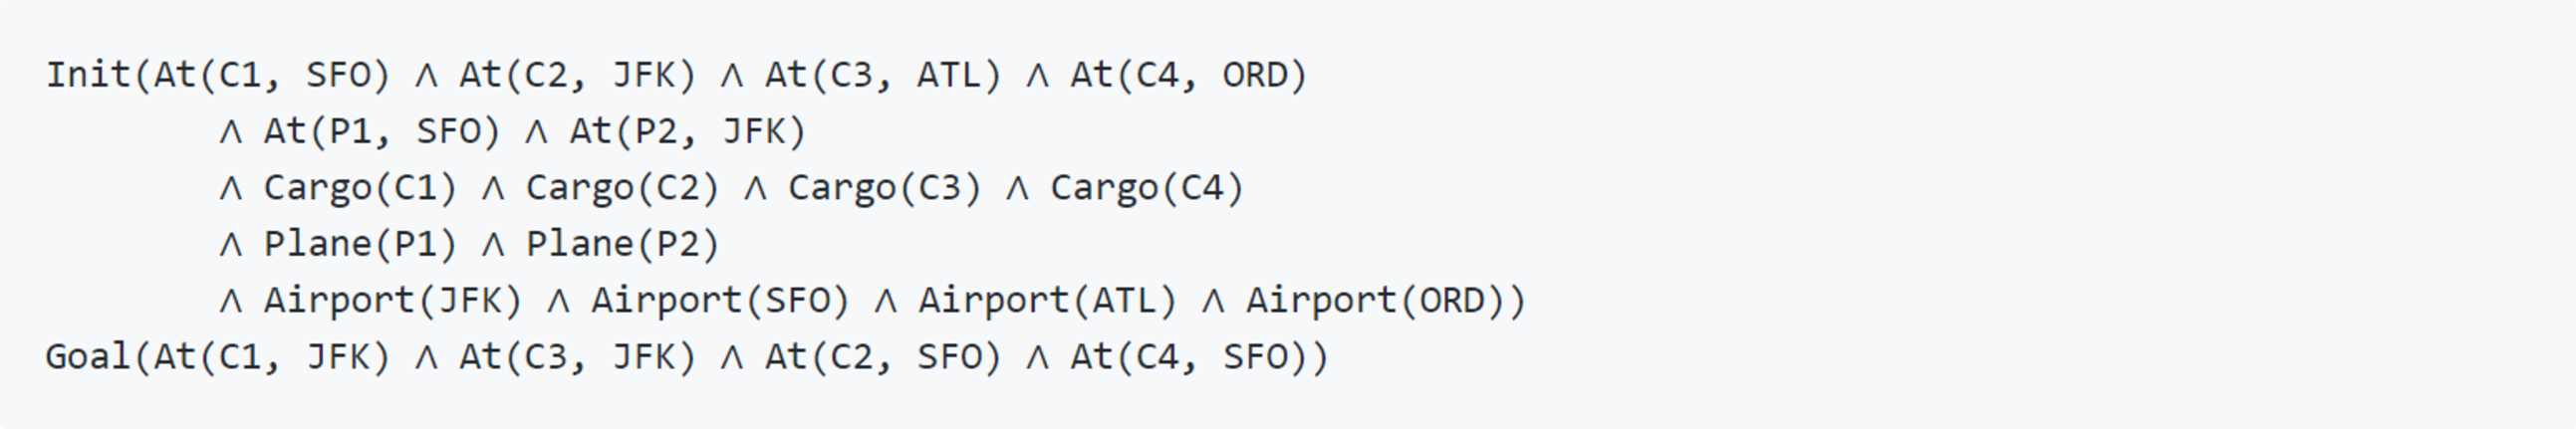
\includegraphics[width=1\linewidth]{problem_3}
		\end{center}
	\end{itemize}
	
	\subsection{Optimal Plan}
	
	A possible optimal plan for each of the aforementioned problems are shown bellow:
	
	\begin{itemize}
		\item Problem 1: 6 steps
		\begin{minted}[
			gobble=3,
			frame=none,
			linenos
			]{yaml}
			Load(C2, P2, JFK)
			Load(C1, P1, SFO)
			Fly(P2, JFK, SFO)
			Unload(C2, P2, SFO)
			Fly(P1, SFO, JFK)
			Unload(C1, P1, JFK)
		\end{minted}
	
		\item Problem 2: 9 steps
		\begin{minted}[
			gobble=3,
			frame=none,
			linenos
			]{yaml}
			Load(C2, P2, JFK)
			Load(C1, P1, SFO)
			Load(C3, P3, ATL)
			Fly(P2, JFK, SFO)
			Unload(C2, P2, SFO)
			Fly(P1, SFO, JFK)
			Unload(C1, P1, JFK)
			Fly(P3, ATL, SFO)
			Unload(C3, P3, SFO)
		\end{minted}
		
		\pagebreak
		
		\item Problem 3: 12 steps
		\begin{minted}[
			gobble=3,
			frame=none,
			linenos
			]{yaml}
			Load(C2, P2, JFK)
			Load(C1, P1, SFO)
			Fly(P2, JFK, ORD)
			Load(C4, P2, ORD)
			Fly(P1, SFO, ATL)
			Load(C3, P1, ATL)
			Fly(P1, ATL, JFK)
			Unload(C1, P1, JFK)
			Unload(C3, P1, JFK)
			Fly(P2, ORD, SFO)
			Unload(C2, P2, SFO)
			Unload(C4, P2, SFO)
		\end{minted}
		
	\end{itemize}

	\section{Planning Search}
	
	Table 1 shows the results for all search methods used to solve the three different versions of the air cargo problem. It compares the non-heuristic search methods (breadth-first-search, breadth-first-tree-search, depth-first-graph-search, depth-limited-search, and uniform-cost-search) and heuristic search methods (recursive-best-first-search, greedy-best-first-graph-search, and Astar-search), which uses a constant as heuristic (h{\_}1, which is not a true heuristic), and two other automatically generated heuristics (ignore-preconditions and planning-graph-level-sum). Note that if the time elapsed to complete the planning search were higher than 10 minutes (600 seconds), the program was interrupted.
	
	\begin{figure}[h]
		\centering
		\caption*{Table 1 - Air Cargo search methods comparison}
		\label{tab:table1}
		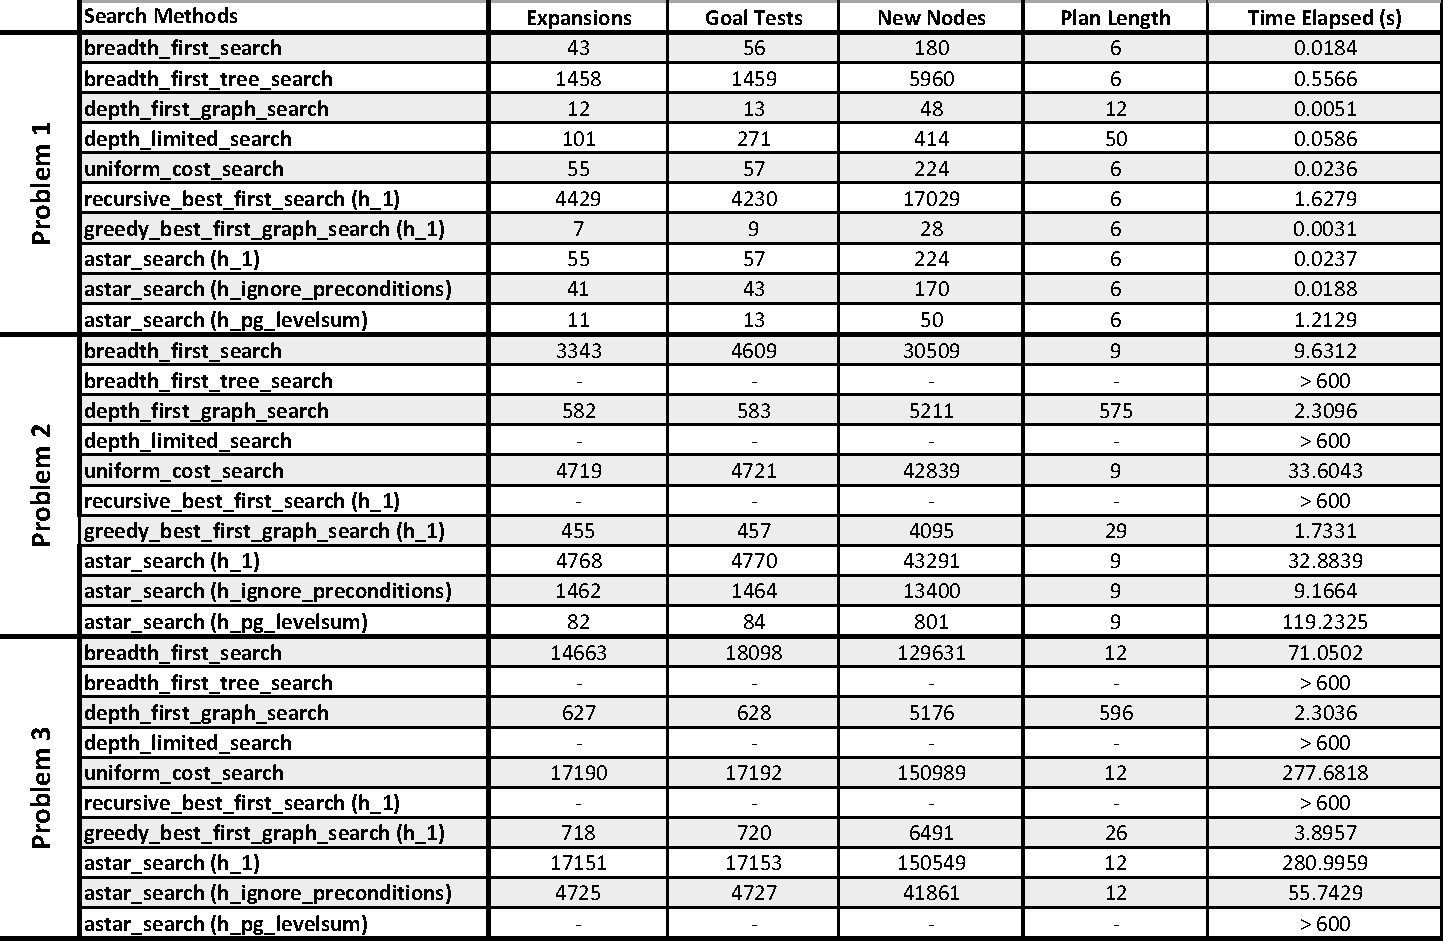
\includegraphics[width=1\linewidth]{Table1}
	\end{figure}

	\subsection{Non-Heuristic Search Methods}
	
	This Section compares the five different non-heuristic search methods present in Table 1. 
	
	The breadth-first-search, breadth-first-tree-search, and the uniform-cost-search methods reached the objective with an optimal plan, as expected. On the other hand, the depth-first-graph-search and the depth-limited-search reached the objective plan, but the plan length was not optimal. 
	
	The breadth-first-search method presented a considerable advantage over the other methods for all problems. Comparing it with the other search methods that achieved an optimal plan, it presented the least number of expansions, goal tests, new nodes formation, and total elapsed time to obtain the plan.
	
	
	\subsection{Heuristic Search Methods}
	
	This Section compares the three different search methods present in Table 1, as well as the different heuristics used.
	
	For problem 1, the best heuristic-based search method was the greedy-best-first-graph-search using the h{\_}1 heuristic. It achieved the optimal plan using the least number of extensions, goal tests, new nodes generation, and time elapsed. Nevertheless, it did not achieved an optimal plan for problems 2 and 3. For these problems, the best method was the Astar-search using the h{\_}ignore{\_}preconditions heuristic, which reached the optimal plan. Although the Astar-search using the h{\_}pg{\_}levelsum presented fewer expansion nodes, goal tests, and new nodes generation, it presented a considerably higher computational burden, which is mainly due to the planning graph construction.
	
	Comparing the Astar-search method using the h{\_}ignore{\_}preconditions heuristic with the breadth-first-search method, it presented fewer expansions, goal tests, and new nodes generation, but it the time elapsed to complete the planning search for both methods varied for each problem. For problem 1, the Astar-search took $0.0188$ seconds against $0.0184$ seconds of the breadth-first-search. For problem 2, the former took $9.1664$ seconds against $9.6312$ seconds of the later. Finally, for problem 3, the former took $55.7429$ seconds against $71.0502$. Therefore, it can be noticed that as the state space grows, more advantageous is the former method comparing to the later.
	
	%\bibliographystyle{plain}
	%\bibliography{Ref}

\end{document}